\documentclass{standalone}
\usepackage{tikz}
\usetikzlibrary{patterns, positioning}


\begin{document}
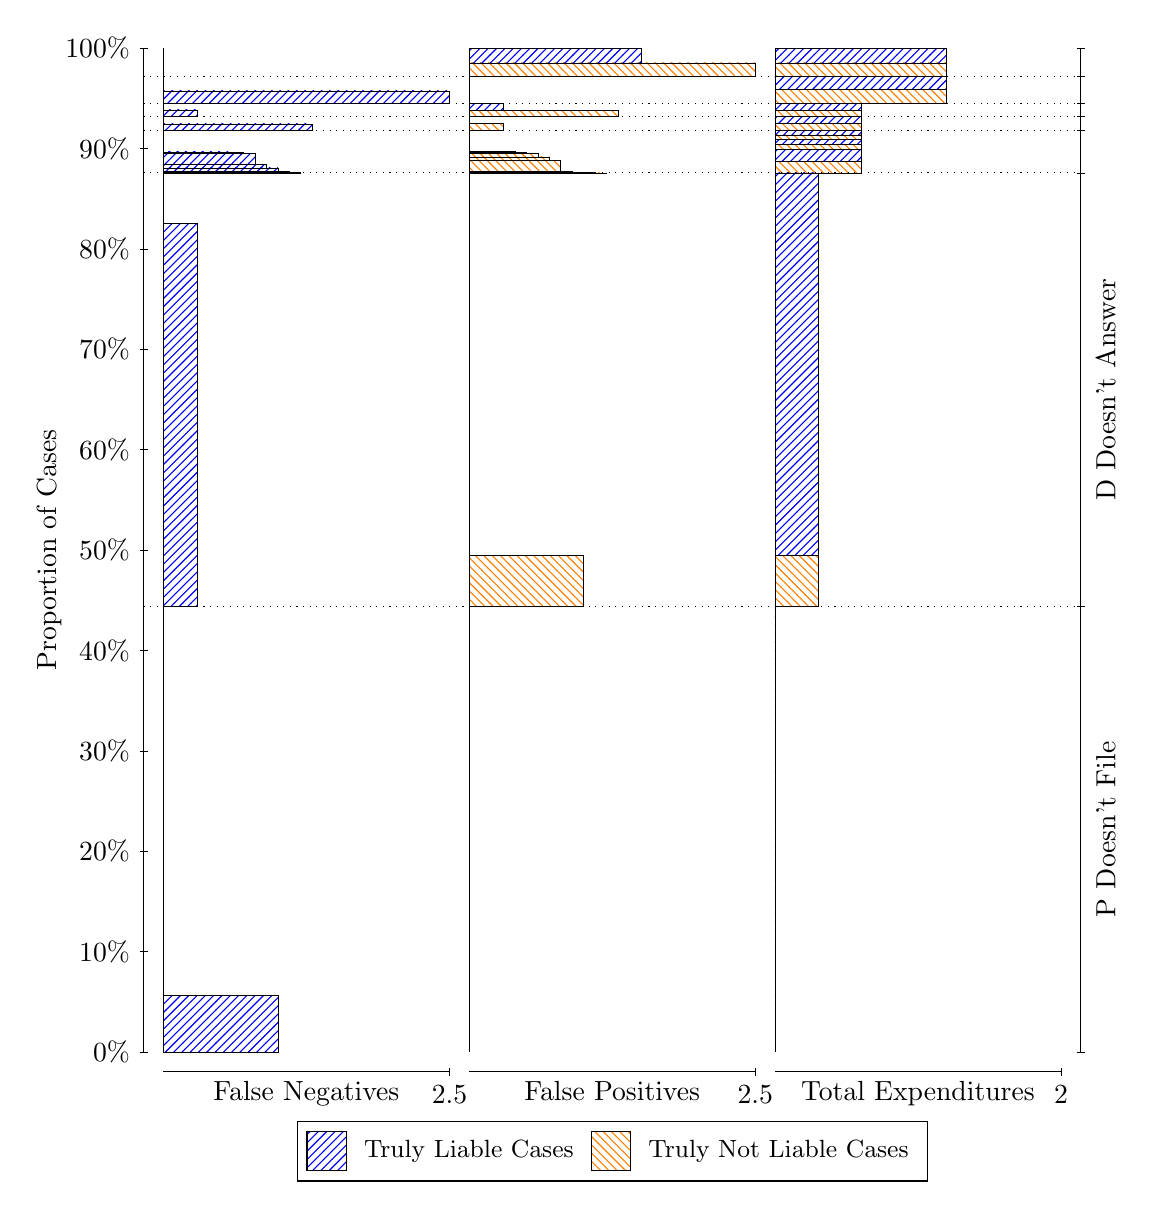
\begin{tikzpicture}
\draw[black, very thin] (1.5,1.75) -- (1.5,14.5);
\node[rotate=90, text=black, anchor=center] at (0.3, 8.125) {Proportion of Cases};
\draw[black, very thin] (1.45,1.75) -- (1.55,1.75);
\node[text=black, anchor=east] at (1.45, 1.75) {0\%};
\draw[black, very thin] (1.45,3.025) -- (1.55,3.025);
\node[text=black, anchor=east] at (1.45, 3.025) {10\%};
\draw[black, very thin] (1.45,4.3) -- (1.55,4.3);
\node[text=black, anchor=east] at (1.45, 4.3) {20\%};
\draw[black, very thin] (1.45,5.575) -- (1.55,5.575);
\node[text=black, anchor=east] at (1.45, 5.575) {30\%};
\draw[black, very thin] (1.45,6.85) -- (1.55,6.85);
\node[text=black, anchor=east] at (1.45, 6.85) {40\%};
\draw[black, very thin] (1.45,8.125) -- (1.55,8.125);
\node[text=black, anchor=east] at (1.45, 8.125) {50\%};
\draw[black, very thin] (1.45,9.4) -- (1.55,9.4);
\node[text=black, anchor=east] at (1.45, 9.4) {60\%};
\draw[black, very thin] (1.45,10.675) -- (1.55,10.675);
\node[text=black, anchor=east] at (1.45, 10.675) {70\%};
\draw[black, very thin] (1.45,11.95) -- (1.55,11.95);
\node[text=black, anchor=east] at (1.45, 11.95) {80\%};
\draw[black, very thin] (1.45,13.225) -- (1.55,13.225);
\node[text=black, anchor=east] at (1.45, 13.225) {90\%};
\draw[black, very thin] (1.45,14.5) -- (1.55,14.5);
\node[text=black, anchor=east] at (1.45, 14.5) {100\%};

\draw[black, very thin] (13.4,1.75) -- (13.4,14.5);
\draw[black, very thin] (13.35,1.75) -- (13.45,1.75);
\node[anchor=west] at (13.35, 1.75) {};
\draw[black, very thin] (13.35,7.4081) -- (13.45,7.4081);
\node[anchor=west] at (13.35, 7.4081) {};
\draw[black, very thin] (13.35,12.914) -- (13.45,12.914);
\node[anchor=west] at (13.35, 12.914) {};
\draw[black, very thin] (13.35,13.45) -- (13.45,13.45);
\node[anchor=west] at (13.35, 13.45) {};
\draw[black, very thin] (13.35,13.63) -- (13.45,13.63);
\node[anchor=west] at (13.35, 13.63) {};
\draw[black, very thin] (13.35,13.792) -- (13.45,13.792);
\node[anchor=west] at (13.35, 13.792) {};
\draw[black, very thin] (13.35,14.143) -- (13.45,14.143);
\node[anchor=west] at (13.35, 14.143) {};
\draw[black, very thin] (13.35,14.5) -- (13.45,14.5);
\node[anchor=west] at (13.35, 14.5) {};

\draw[black, very thin, pattern color=blue, pattern=north east lines] (1.75,1.75) rectangle (3.2033,2.4694);
\draw[black, very thin, pattern color=orange, pattern=north west lines] (1.75,2.4694) rectangle (1.75,7.4081);
\draw[black, very thin, pattern color=blue, pattern=north east lines] (1.75,7.4081) rectangle (2.186,12.27);
\draw[black, very thin, pattern color=orange, pattern=north west lines] (1.75,12.27) rectangle (1.75,12.914);
\draw[black, very thin, pattern color=blue, pattern=north east lines] (1.75,12.914) rectangle (3.494,12.923);
\draw[black, very thin, pattern color=blue, pattern=north east lines] (1.75,12.923) rectangle (3.3487,12.934);
\draw[black, very thin, pattern color=blue, pattern=north east lines] (1.75,12.934) rectangle (3.2033,12.978);
\draw[black, very thin, pattern color=blue, pattern=north east lines] (1.75,12.978) rectangle (3.058,12.979);
\draw[black, very thin, pattern color=blue, pattern=north east lines] (1.75,12.979) rectangle (3.058,13.021);
\draw[black, very thin, pattern color=blue, pattern=north east lines] (1.75,13.021) rectangle (2.9127,13.165);
\draw[black, very thin, pattern color=blue, pattern=north east lines] (1.75,13.165) rectangle (2.7673,13.175);
\draw[black, very thin, pattern color=blue, pattern=north east lines] (1.75,13.175) rectangle (2.622,13.18);
\draw[black, very thin, pattern color=blue, pattern=north east lines] (1.75,13.18) rectangle (2.4767,13.18);
\draw[black, very thin, pattern color=blue, pattern=north east lines] (1.75,13.18) rectangle (2.3313,13.182);
\draw[black, very thin, pattern color=orange, pattern=north west lines] (1.75,13.182) rectangle (1.75,13.45);
\draw[black, very thin, pattern color=blue, pattern=north east lines] (1.75,13.45) rectangle (3.6393,13.536);
\draw[black, very thin, pattern color=orange, pattern=north west lines] (1.75,13.536) rectangle (1.75,13.63);
\draw[black, very thin, pattern color=blue, pattern=north east lines] (1.75,13.63) rectangle (2.186,13.714);
\draw[black, very thin, pattern color=orange, pattern=north west lines] (1.75,13.714) rectangle (1.75,13.792);
\draw[black, very thin, pattern color=blue, pattern=north east lines] (1.75,13.792) rectangle (5.3833,13.957);
\draw[black, very thin, pattern color=orange, pattern=north west lines] (1.75,13.957) rectangle (1.75,14.143);
\draw[black, very thin, pattern color=orange, pattern=north west lines] (1.75,14.143) rectangle (1.75,14.31);
\draw[black, very thin, pattern color=blue, pattern=north east lines] (1.75,14.31) rectangle (1.75,14.5);
\draw[black, very thin, pattern color=orange, pattern=north west lines] (5.6333,1.75) rectangle (5.6333,6.6886);
\draw[black, very thin, pattern color=blue, pattern=north east lines] (5.6333,6.6886) rectangle (5.6333,7.4081);
\draw[black, very thin, pattern color=orange, pattern=north west lines] (5.6333,7.4081) rectangle (7.0867,8.0521);
\draw[black, very thin, pattern color=blue, pattern=north east lines] (5.6333,8.0521) rectangle (5.6333,12.914);
\draw[black, very thin, pattern color=orange, pattern=north west lines] (5.6333,12.914) rectangle (7.3773,12.915);
\draw[black, very thin, pattern color=orange, pattern=north west lines] (5.6333,12.915) rectangle (7.232,12.916);
\draw[black, very thin, pattern color=orange, pattern=north west lines] (5.6333,12.916) rectangle (7.0867,12.92);
\draw[black, very thin, pattern color=orange, pattern=north west lines] (5.6333,12.92) rectangle (6.9413,12.93);
\draw[black, very thin, pattern color=orange, pattern=north west lines] (5.6333,12.93) rectangle (6.796,13.074);
\draw[black, very thin, pattern color=orange, pattern=north west lines] (5.6333,13.074) rectangle (6.6507,13.118);
\draw[black, very thin, pattern color=orange, pattern=north west lines] (5.6333,13.118) rectangle (6.5053,13.162);
\draw[black, very thin, pattern color=orange, pattern=north west lines] (5.6333,13.162) rectangle (6.36,13.172);
\draw[black, very thin, pattern color=orange, pattern=north west lines] (5.6333,13.172) rectangle (6.2147,13.183);
\draw[black, very thin, pattern color=blue, pattern=north east lines] (5.6333,13.183) rectangle (5.924,13.184);
\draw[black, very thin, pattern color=blue, pattern=north east lines] (5.6333,13.184) rectangle (5.7787,13.185);
\draw[black, very thin, pattern color=blue, pattern=north east lines] (5.6333,13.185) rectangle (5.6333,13.45);
\draw[black, very thin, pattern color=orange, pattern=north west lines] (5.6333,13.45) rectangle (6.0693,13.544);
\draw[black, very thin, pattern color=blue, pattern=north east lines] (5.6333,13.544) rectangle (5.6333,13.63);
\draw[black, very thin, pattern color=orange, pattern=north west lines] (5.6333,13.63) rectangle (7.5227,13.707);
\draw[black, very thin, pattern color=blue, pattern=north east lines] (5.6333,13.707) rectangle (6.0693,13.792);
\draw[black, very thin, pattern color=orange, pattern=north west lines] (5.6333,13.792) rectangle (5.6333,13.978);
\draw[black, very thin, pattern color=blue, pattern=north east lines] (5.6333,13.978) rectangle (5.6333,14.143);
\draw[black, very thin, pattern color=orange, pattern=north west lines] (5.6333,14.143) rectangle (9.2667,14.31);
\draw[black, very thin, pattern color=blue, pattern=north east lines] (5.6333,14.31) rectangle (7.8133,14.5);
\draw[black, very thin, pattern color=orange, pattern=north west lines] (9.5167,1.75) rectangle (9.5167,6.6886);
\draw[black, very thin, pattern color=blue, pattern=north east lines] (9.5167,6.6886) rectangle (9.5167,7.4081);
\draw[black, very thin, pattern color=orange, pattern=north west lines] (9.5167,7.4081) rectangle (10.062,8.0521);
\draw[black, very thin, pattern color=blue, pattern=north east lines] (9.5167,8.0521) rectangle (10.062,12.914);
\draw[black, very thin, pattern color=orange, pattern=north west lines] (9.5167,12.914) rectangle (10.607,13.063);
\draw[black, very thin, pattern color=blue, pattern=north east lines] (9.5167,13.063) rectangle (10.607,13.212);
\draw[black, very thin, pattern color=orange, pattern=north west lines] (9.5167,13.212) rectangle (10.607,13.278);
\draw[black, very thin, pattern color=blue, pattern=north east lines] (9.5167,13.278) rectangle (10.607,13.343);
\draw[black, very thin, pattern color=orange, pattern=north west lines] (9.5167,13.343) rectangle (10.607,13.396);
\draw[black, very thin, pattern color=blue, pattern=north east lines] (9.5167,13.396) rectangle (10.607,13.45);
\draw[black, very thin, pattern color=orange, pattern=north west lines] (9.5167,13.45) rectangle (10.607,13.544);
\draw[black, very thin, pattern color=blue, pattern=north east lines] (9.5167,13.544) rectangle (10.607,13.63);
\draw[black, very thin, pattern color=orange, pattern=north west lines] (9.5167,13.63) rectangle (10.607,13.707);
\draw[black, very thin, pattern color=blue, pattern=north east lines] (9.5167,13.707) rectangle (10.607,13.792);
\draw[black, very thin, pattern color=orange, pattern=north west lines] (9.5167,13.792) rectangle (11.697,13.978);
\draw[black, very thin, pattern color=blue, pattern=north east lines] (9.5167,13.978) rectangle (11.697,14.143);
\draw[black, very thin, pattern color=orange, pattern=north west lines] (9.5167,14.143) rectangle (11.697,14.31);
\draw[black, very thin, pattern color=blue, pattern=north east lines] (9.5167,14.31) rectangle (11.697,14.5);
\draw[black, dotted] (1.5,7.4081) -- (13.4,7.4081);
\draw[black, dotted] (1.5,12.914) -- (13.4,12.914);
\draw[black, dotted] (1.5,13.45) -- (13.4,13.45);
\draw[black, dotted] (1.5,13.63) -- (13.4,13.63);
\draw[black, dotted] (1.5,13.792) -- (13.4,13.792);
\draw[black, dotted] (1.5,14.143) -- (13.4,14.143);
\draw[black, very thin] (1.75,1.5) -- (5.3833,1.5);
\node[text=black, anchor=north] at (3.5667, 1.5) {False Negatives};
\draw[black, very thin] (5.3833,1.45) -- (5.3833,1.55);
\node[text=black, anchor=north] at (5.3833, 1.45) {2.5};

\draw[black, very thin] (5.6333,1.5) -- (9.2667,1.5);
\node[text=black, anchor=north] at (7.45, 1.5) {False Positives};
\draw[black, very thin] (9.2667,1.45) -- (9.2667,1.55);
\node[text=black, anchor=north] at (9.2667, 1.45) {2.5};

\draw[black, very thin] (9.5167,1.5) -- (13.15,1.5);
\node[text=black, anchor=north] at (11.333, 1.5) {Total Expenditures};
\draw[black, very thin] (13.15,1.45) -- (13.15,1.55);
\node[text=black, anchor=north] at (13.15, 1.45) {2};

\node[text=black, centered, rotate=90] at (13.72, 4.579) {P Doesn't File};
\node[text=black, centered, rotate=90] at (13.72, 10.161) {D Doesn't Answer};






\draw (7.449999999999999,1.5) node[draw=none] (baseCoordinate) {};
\begin{scope}[align=center]
        \matrix[scale=0.5, draw=black, below=0.5cm of baseCoordinate, nodes={draw}, column sep=0.1cm]{
            \node[rectangle, draw, minimum width=0.5cm, minimum height=0.5cm, pattern color=blue, pattern=north east lines] {}; &
            \node[draw=none, font=\small, text=black] (B) {Truly Liable Cases}; &
            \node[rectangle, draw, minimum width=0.5cm, minimum height=0.5cm, pattern color=orange, pattern=north west lines] {}; &
            \node[draw=none, font=\small, text=black] (B) {Truly Not Liable Cases}; \\
            };
\end{scope}

\end{tikzpicture}
\end{document}